% Compact PGFPlots panel for sampled surface11 BSC GEXIT derivative.
% Requires \usepackage{pgfplots} and \pgfplotsset{compat=1.18}.
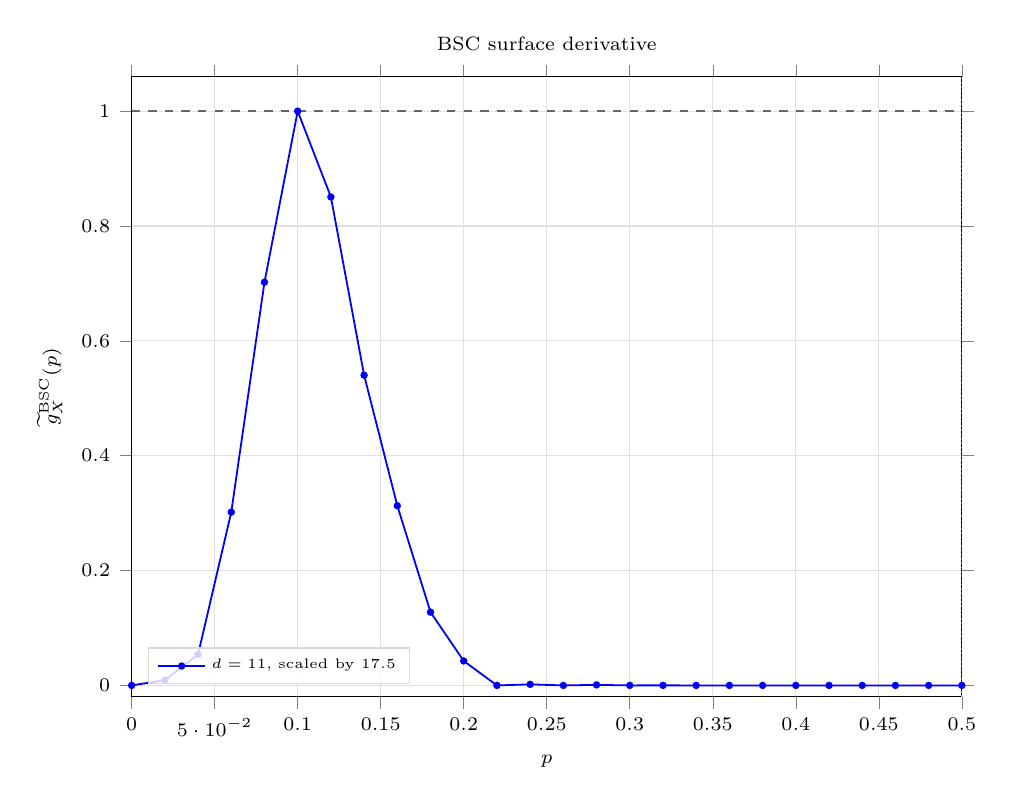
\begin{tikzpicture}
\begin{axis}[
  name=scaledBSCGEXITSurface11Axis,
  width=\linewidth,
  height=0.78\linewidth,
  title={BSC surface derivative},
  title style={font=\scriptsize},
  xlabel={$p$},
  ylabel={$\widetilde g_X^{\rm BSC}(p)$},
  xmin=0, xmax=0.5,
  ymin=-0.02, ymax=1.06,
  grid=both,
  major grid style={black!12},
  minor grid style={black!6},
  tick align=outside,
  tick label style={font=\scriptsize},
  label style={font=\scriptsize},
  legend cell align={left},
  legend style={draw=black!15, fill=white, fill opacity=0.82, text opacity=1, at={(0.02,0.02)}, anchor=south west, font=\tiny},
]
\addplot[black!60, densely dotted, line width=0.55pt, forget plot] coordinates {(0.5,-0.02) (0.5,1.06)};
\addplot[black!60, dashed, line width=0.55pt, forget plot] coordinates {(0,1) (0.5,1)};
\addplot+[color=blue, mark=*, mark size=1.0pt, line width=0.65pt]
coordinates {(0,0) (0.02,0.00913744739745) (0.04,0.0538532186741) (0.06,0.301791394672) (0.08,0.702172954844) (0.1,1) (0.12,0.850636257303) (0.14,0.540355065678) (0.16,0.312897872887) (0.18,0.127632529059) (0.2,0.0425813400342) (0.22,0) (0.24,0.00184556440935) (0.26,0) (0.28,0.00094824548566) (0.3,2.549588016e-05) (0.32,7.68991804109e-05) (0.34,0) (0.36,0) (0.38,7.4608288285e-08) (0.4,0) (0.42,6.82762707509e-09) (0.44,2.92109545967e-10) (0.46,1.67385314544e-11) (0.48,0) (0.5,0)};
\addlegendentry{$d=11$, scaled by $17.5$}
\end{axis}
\end{tikzpicture}
